\documentclass[journal=nalefd,manuscript=letter]{achemso}
\setkeys{acs}{articletitle=true}
\usepackage{graphicx}
\usepackage{amsmath}
\usepackage{amssymb}
\usepackage{subfigure}
\usepackage{xr}
%%% This is for adding a footer with the time of the compilation of the file.
%%% Useful for versioning of printed copies.
\usepackage{datetime}
\usepackage{fancyhdr}
\fancyfoot[L]{\fontsize{8}{12} \selectfont \today $\,$ \currenttime}
\pagestyle{fancy}
%%%%%%%%%%%%%%%%%%%%%%%%%%%%%%%%%%%%%%%%%%%%%%%%%%%%%%%%%%%%%%%%%%%%%
%%%%%%%%%%%%%%%%%%%%%%%%%%%%%%%%%%%%%%%%%%%%%%%%%%%%%%%%%%%%%%%%%%%%%

\usepackage[version=3]{mhchem} % Formula subscripts using \ce{}
\usepackage[T1]{fontenc}       % Use modern font encodings
\externaldocument{supporting}

\newcommand{\K}{\ensuremath{\,\textrm{K}}}
\newcommand{\nm}{\ensuremath{\,\textrm{nm}}}
\newcommand{\mm}{\ensuremath{\,\textrm{mm}}}
\newcommand{\um}{\ensuremath{\,\mu\textrm{m}}}
\newcommand{\eV}{\ensuremath{\,\textrm{eV}}}
\newcommand{\uM}{\ensuremath{\,\mu\textrm{M}}}
\newcommand{\uW}{\ensuremath{\,\mu\textrm{W}}}
\newcommand{\mW}{\ensuremath{\,\textrm{mW}}}
\newcommand{\pM}{\ensuremath{\,\textrm{pM}}}
\newcommand{\meV}{\ensuremath{\,\textrm{meV}}}
\newcommand{\pwr}{\ensuremath{\,\textrm{kW/cm}^2}}
\newcommand{\fs}{\ensuremath{\,\textrm{fs}}}
\newcommand{\ps}{\ensuremath{\,\textrm{ps}}}
\newcommand{\CPS}{\ensuremath{\,\textrm{CPS}}}
\newcommand{\kCPS}{\ensuremath{\,\textrm{kCPS}}}
\newcommand{\atto}{\ensuremath{\textrm{ATTO}\,647\textrm{N}}}


\author{Aquiles Carattino}
\affiliation[Leiden]
{Huygens-Kamerlingh Onnes Lab, 2300RA Leiden, The Netherlands}
\author{Michel Orrit}
\email{orrit@physics.leidenuniv.nl}
\affiliation[Leiden]
{Huygens-Kamerlingh Onnes Lab, 2300RA Leiden, The Netherlands}

\title{Gold nanoparticles as nano-thermometers}

\keywords{Gold nanorods, Plasmon, Anti-Stokes, Sensing, Temperature}

\begin{document}
\maketitle
\abstract{This is the abstract}
\section{Introduction}
Most physical, chemical, biological processes depend on temperature. Together
with the miniaturization of devices and the advent of nanotechnology the need
for measuring temperature with high spatial accuracy started to emerge. Notably
in biology\cite{Yang2011a,Hrelescu2010} and medicine\cite{Li2013c}
measuring and controlling temperature at a single cell level will provide not only insight into
intracellular processes but it will also contribute to a better understanding of
the mechanisms involved in the proposed new therapies such as photothermal tumor
ablation\cite{Gobin2007} or controlled drug
delivery\cite{Huang2006}\cite{Huo2014}.

Probes with distinctive spectral features are ideal candidates for temperature
measurements since they provide high spatial accuracy while far field optics
allow a non contact readout. Some of the proposed strategies include structures
that undergo a conformational change upon a change in
temperatures\cite{Ebrahimi2014}, thus inducing a change in fluorescence
intensity of a dye molecule embedded into them. Also cleverly designed
fluorescent probes\cite{Vetrone2010} in which the ratio of particular emission
peaks depends on temperature allow a high accuracy and can be used for
intracellular thermometry.

The use of anti-Stokes fluorescence emission from lanthanide ions has been
studied for several years\cite{Auzel2004a} and can be used to determine
temperature with high accuracy. However organic dyes show a very low amount of
emitted photons with a higher energy than the excitation energy, rendering their
use in biological conditions very challenging. Recently Surface Enhanced Raman
Spectroscopy (SERS) allowed to measure changes induced by temperature down
to single molecules\cite{Pozzi2015}, but a careful calibration of the
measurements is crucial.

At a cellular level measuring temperature has been subject to extensive
debates\cite{Yang2011a,Suzuki2015}. Many cellular processes may be subject to
temperature variations, including heat generation at mitochondria. However the
measured temperatures\cite{Yang2011} are in the order of $10^5$ times higher
than the expected values drawn from theoretical models\cite{Sato2014}.
Moreover new applications in photothermal therapy require locally increasing the
temperature in order to induce the death of specific cells in a
tissue\cite{Huang2008,Huang2006}. Many of these methods employ metallic
nanoparticles as heat sources\cite{Gobin2007,Hirsch2003} but rely on
models\cite{Zhao2014a} or on ad-hoc calibrations to estimate the temperatures
reached\cite{Donner2013}. Therefore a method that allows both to increase the
local temperature and to monitor it will be of great interest in a broad range
of fields.

Gold nanoparticles continue to receive a great amount of attention because of
their optical properties\cite{Zijlstra2011}. A large absorption and scattering
cross section spanning through almost the entire visible spectrum makes them
easy to detect via exciting their luminescence and collecting either the Stokes
or the anti-Stokes emission\cite{Jiang2013}; in a dark field
scattering\cite{Hu2008} configuration or via photothermal
imaging\cite{Berciaud2006}. Moreover their signal is stable over time; gold
nanoparticles do not blink nor bleach, making them ideal candidates for
biological labeling.

Different metallic nano-objects are being introduced as agents for photothermal
therapy or drug delivery\cite{Kang2013}. One of the advantages of gold
nanoparticles is the possibility of tuning their resonance to the near infra-red
range, where the penetration of light into tissues can be of several
centimeters\cite{Huang2006,Gobin2007,Hirsch2003,ONeal2004,Li2013c,Huang2008}.
Moreover the particles can be used not only for treatment, but also for imaging.
In this work we propose that the anti-Stokes luminescence of gold nanorods and
nanospheres can be used to measure their temperature with a relatively high
accuracy.

Luminescence of metallic nanoparticles has been object of extensive study in
recent years. Since the first observation of luminescence from bulk
gold\cite{Mooradian1969}, different groups have tried to quantitatively describe
the observed properties\cite{Mohamed2000,Beversluis2003a}, as the quantum
yield\cite{Fang2012,Rao2015,Yorulmaz2012,Cheng2015} and the emission
spectrum\cite{Link2010}. Several computer packages\cite{Yurkin2011} allow to
compute the cross sections of different geometries and there are already several successful
applications of nanoparticles into different fields. The anti-Stokes emission
from these particles has however been largely overlooked.

The mechanism we propose to explain the luminescence from gold nanoparticles is
based in the radiative recombination of electron and holes that are created upon
the absorption of an incident photon\cite{Dulkeith2004,Mooradian1969}. The
emission will be enhanced by the presence of the surface plasmon acting as an
antenna\cite{Mohamed2000}. At the same time, the probability of the interaction
of the electron or hole with a phonon before recombining can give rise to an
emission photon with a higher energy than the
excitation\cite{Hodak2000,Giri2015,Arbouet2003a}.

A monochromatic photon incident to the particle will give rise to a collective
oscillation of the gas of conduction electrons. The coherence of the oscillation
is broken due to collisions with the particle's surface and to the interaction
with baths\cite{Zhao2016,Sonnichsen2002}. These can be mainly the
electron-electron interactions, electron-phonon coupling and the bath of photons
coupled via spontaneous emission. The decoherence time can be measured in pulsed
experiments or deduced from the inverse linewidth of the plasmon resonance and
is in the order of $6\fs$ or shorter\cite{Sun1994}. After this the state of the
system can be described as a superposition of hot electron and hole states.

The hot electron and hole cool down by exchanging energy with the lattice on a
timescale of $\tau\approx1\ps$\cite{Pustovalov2005}. Before this happens,
electron and hole have a small probability of recombining radiatively,
re-emitting their high electronic energy as a photoluminescence photon. If they
have interacted only with static surfaces, their energy would be the same and
therefore the emitted photon would have the same energy than the incoming
photon, and will not contribute to the measured photoluminescence (will be
blocked by the notch filter.) If on the other hand they have interacted with a
phonon they have lost or acquired a phonon energy and momentum quantum before
recombining.

Electron and hole can also interact with phonons upon recombination, either by
creation or annihilaton of a phonon. In both cases the energy available upon
recombination cannot exceed $\hbar\omega_L+k_BT$. It has to be noted that in the
hypothesis of a single-photon absorption, i.e. at low excitation power, the
temperature $T$ is that of the bath before absorption, the temperature of the
surrounding medium of the particle. This is different from pulsed experiments,
in which the electron gas temperature can be orders of magnitude higher than
room temperature\cite{Baffou2013a}. 

Radiative recombination gives rise to weakly emitting sources spatially and
spectrally distributed throughout the particle over a broad frequency band with
an exponential cutoff at $\hbar\omega_\textrm{L}+k_\textrm{B}T$. The weak
recombination emission can be greatly enhanced by the surface plasmon resonance,
acting as an antenna. With this model the following prediction can be made.
Firstly the emission spectrum must follow the plasmon spectrum if the excitation
laser is well above the plasmon resonance as shown in Figure
\ref{fig:spectra_rod} in the results. If the excitation falls within the
plasmon resonance, the spectrum is expected to follow the plasmon spectrum multiplied by
Bose-Einstein statistics factor arising from phonon population.
This factor should be proportional to $\bar{n}$ for anti-Stokes and $\bar{n}+1$
for Stokes processes, where

\begin{equation}
	\bar{n}=\left(\exp\frac{\hbar\Omega}{k_bT}-1\right)^{-1}.
\end{equation}

With this model, it can also be predicted that the emission should be polarized
as the plasmon; for gold nanorods this polarization coincides with the
longitudinal axis of the particle\cite{He2015}. Moreover, the lifetime should be
determined by the lifetime of hot electrons and holes and should be
significatively shorter than the thermalization time of the carriers. If this
was not the case, few interactions with phonons are enough to reduce the
carriers' energy and therefore the electron and hole wouldn't have enough energy
to produce an optical photon. Finally in the model only the presence of hot
carriers is required. As the wavevectors are randomly distributed at all times,
the recombination probability remains constant at all stages of relaxation.
Therefore excitation well above the plasmon resonance should excite the
photoluminescence with nearly the same efficiency as just above the plasmon
resonance.

In this work we propose to use the anti-Stokes luminescence emission from gold
nanoparticles to determine their temperature. According to the model just
described, the anti-Stokes emission follows the following form,
\begin{equation}\label{eqn:fitting}
	I(\nu) =
	\textrm{SPR}(\nu)\cdot\left(\exp\frac{\textrm{h}(\nu-\nu_L)}{k_\textrm{B}T}-1\right)^{-1}
\end{equation}
where $I$ is the intensity, $\nu$ is the frequency of the photons, $SPR$ is the
surface plasmon resonance, $\nu_L$ is the frequency of the laser, $h$ is
Planck's constant, $k_\textrm{B}$ the Boltzmann constant and the only remaining
free parameter is the Temperature $T$ (plus a normalization constant not
included in eqn. \ref{eqn:fitting}.) This means that carefully fitting the
emission spectra allows to extract the absolute temperature of the
particles without any previous calibration.

\section{Experimental method}
All the measurements in this work were performed in a home-built confocal
microscope equipped with an APD and a spectrometer (Acton 500i). Samples were
mounted in a flowcell that allowed to increase the temperature of the medium up
to $60\,^oC$ and to monitor it through a Pt100 resistance thermometer placed
$1\mm$ away from the observation area.

Samples were prepared by spin casting a suspension of nanoparticles onto clean
coverslips. Different particles were employed in this work. Nanorods with
average dimensions of $21\nm\times50\nm$ and a plasmon resonance around $650\nm$
were synthesized following the seeded-growth method; spheres with radii between
$30\nm$ and $60\nm$ were purchased from BBI International. We employed a
$532\nm$ (CNI) laser for characterizing the nanorods' plasmon and for exciting
spheres close to resonance. A $633\nm$ HeNe (Thorlabs) was employed to excite
the nanorods in resonance.

Room temperature measurements were performed using a $60X$, NA $1.4$ oil
immersion objective (Olympus). This allowed a high excitation and collection
efficiency. At higher temperatures a dry objective, $60X$, NA $0.9$ (Olympus)
was employed to avoid the presence of a heat-sink directly in contact to the
observed area. The lower NA of this objective made both the excitation and
collection efficiencies significantly lower. The first can be compensated
increasing the excitation power, the latter however is inherent to the method
and can be compensated by increasing the exposure time.

To compensate for the drift of the setup while increasing the temperature, a
computer program was developed to continuously track a reference particle. The
same program was responsible for recording the temperature and triggering the
spectrometer. In this way complete data sets were acquired at different
temperatures, including spectra while exciting at $532\nm$, at $633\nm$ with
different laser intensities and the temperature measured by the Pt100. A
spectrum with the $532\nm$ laser was taken after every cycle to ensure that the
particle was not reshaping due to higher excitation powers.

The intensity of the lasers was controlled via the voltage applied to an AOM in
each optical path. Several accumulations of the spectra at the same laser
intensity were recorded. On one hand this allowed to lower the noise of the
measurements. On the other also allowed to remove bright pixels generated by
cosmic rays and to monitor changes in the intensity of the spectra during the
acquisition. These changes can be due to a drift of the setup while measuring or
to a reshape of the particle, that can be confirmed by comparing the spectra
acquired with the $532\nm$ laser. In case of a recorded intensity change larger
than acceptable, the particular spectra was disregarded.

To calculate the heating of the particles the absorption cross section has to be
computed. For the case of nanorods, the ADDA package was employed. Spheres'
cross section can be calculated from Mie theory. Once the dissipated power is
known, the parameters can be either used in a Comsol model or the
heat equation can be analytically solved, approximating the rods by spheres of
the same volume.

\section{Results}
\begin{figure}[htp] \centering
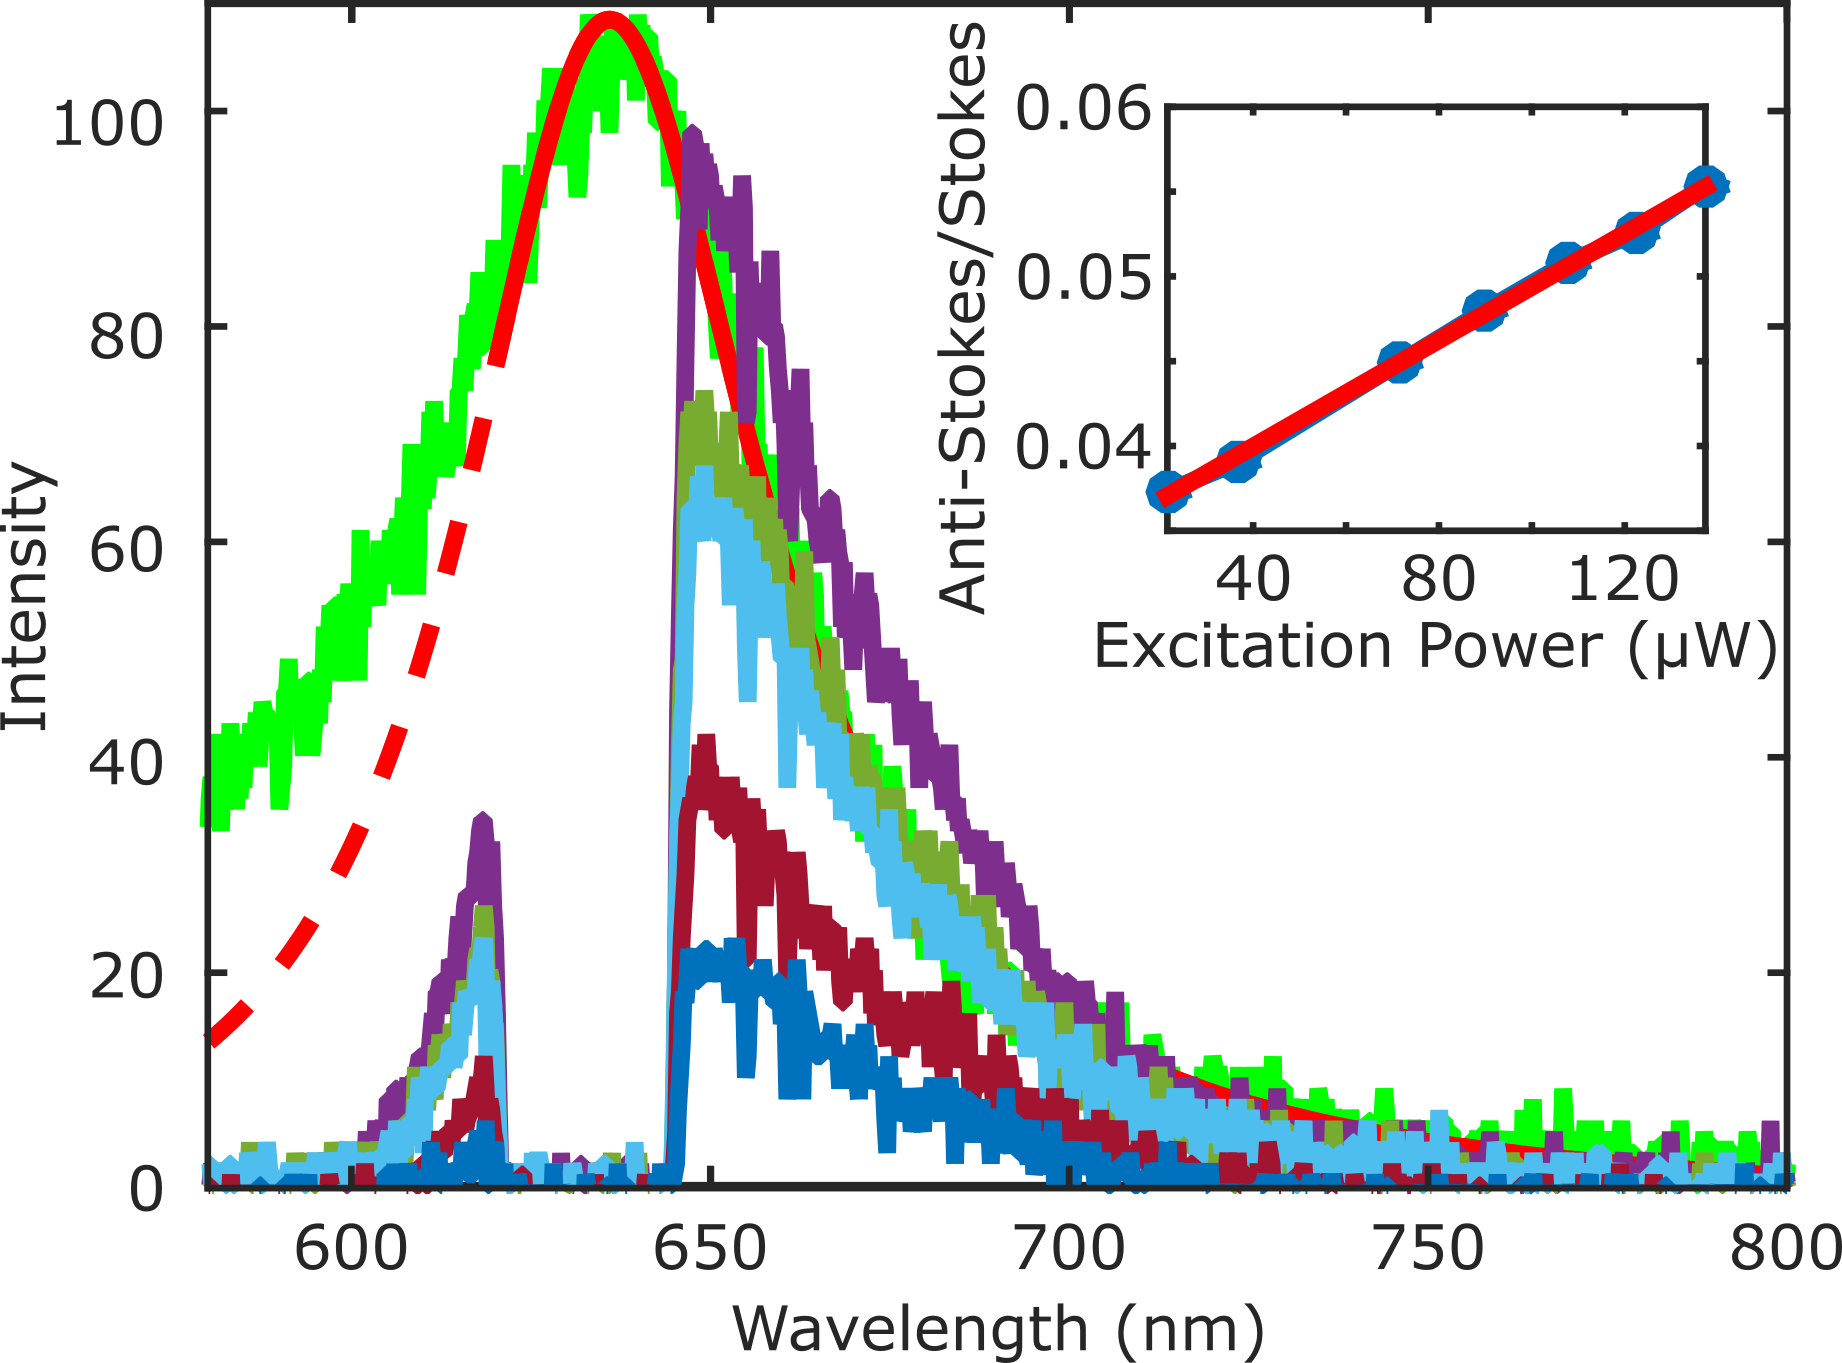
\includegraphics[width=0.45\textwidth]{Figures/02_Several_Intensities/02_several_intensities.png}
\caption{Luminescence spectra of a single gold nanorod. The green curve is the
emission under $532\nm$ excitation. In red is the fitting by a lorentzian; the
dashed part is the region that was not considered for the fitting. The other
curves are the emission of the same particle under $633\nm$ irradiation at five 
different powers. The inset shows the anti-Stokes-to-Stokes ratio as a function
of the excitation power, overlapped with a linear fit in red.}
	\label{fig:spectra_rod}
\end{figure}

The proposed model for the anti-Stokes emission requires to know the plasmon
spectrum ($SPR$ function in equation \ref{eqn:fitting}) of the particle in order
to fit the emission at shorter wavelengths and extract its temperature. It has
been shown that both scattering and luminescence spectra overlap over a broad
range of wavelengths\cite{Yorulmaz2012}. Therefore exciting gold nanorods with
$532\nm$ allows to record the longitudinal plasmon spectra, as shown in the
green solid curve of Figure \ref{fig:spectra_rod}. The peak was fitted by a
single lorentzian, shown in red in the Figure; the dashed part of the curve
depicts the spectral region that was not considered for the fitting. It has to
be reminded that the luminescence spectra is not a perfect lorentzian since
there is a broadband contribution to the lumienscence arising between the
excitation wavelength and the plasmon peak\cite{Boyd1986}. This appears as an
asymmetry in the emission spectrum, particularly visible for wavelengths smaller
than $625\nm$. The results of this fitting will be employed for the SPR function
defined in equation \ref{eqn:fitting}. A lengthier discussion on the effects of
this procedure will be given later.

The other curves in Fig. \ref{fig:spectra_rod} show the luminescence emission of
the same nanorod while irradiating with a $633\nm$ laser at different powers,
ranging from $25\uW$ to $125\uW$ at the back aperture of the objective. The
vertical black line shows the wavelength of the laser. The Stokes part of the
spectrum at longer wavelengths than the excitation, show the same shape than the
plasmon emission observed under $532\nm$ excitation, besides for a normalization
factor. From the figure it can readily be seen that the shape of the anti-Stokes
emission, at shorter wavelengths than excitation, is exponential-like and
doesn't follow the lorentzian shape of the Stokes emission. The dip between
Stokes and anti-Stokes is caused by the notch filter that prevents direct
excitation light from reaching the detectors.

The inset of Fig. \ref{fig:spectra_rod} shows the anti-Stokes-to-Stokes ratio of
the integrated luminescence for different laser excitation intensities. It is
possible to see that even with a linear behavior, the anti-Stokes intensity
increases more rapidly with laser excitation power than the Stokes emission.
This phenomenon was already exploited to image gold nanorods in high-background
conditions. Moreover it shows that the anti-Stokes emission depends on
laser excitation power differently than its Stokes counterpart. 

\begin{figure}[htp] \centering
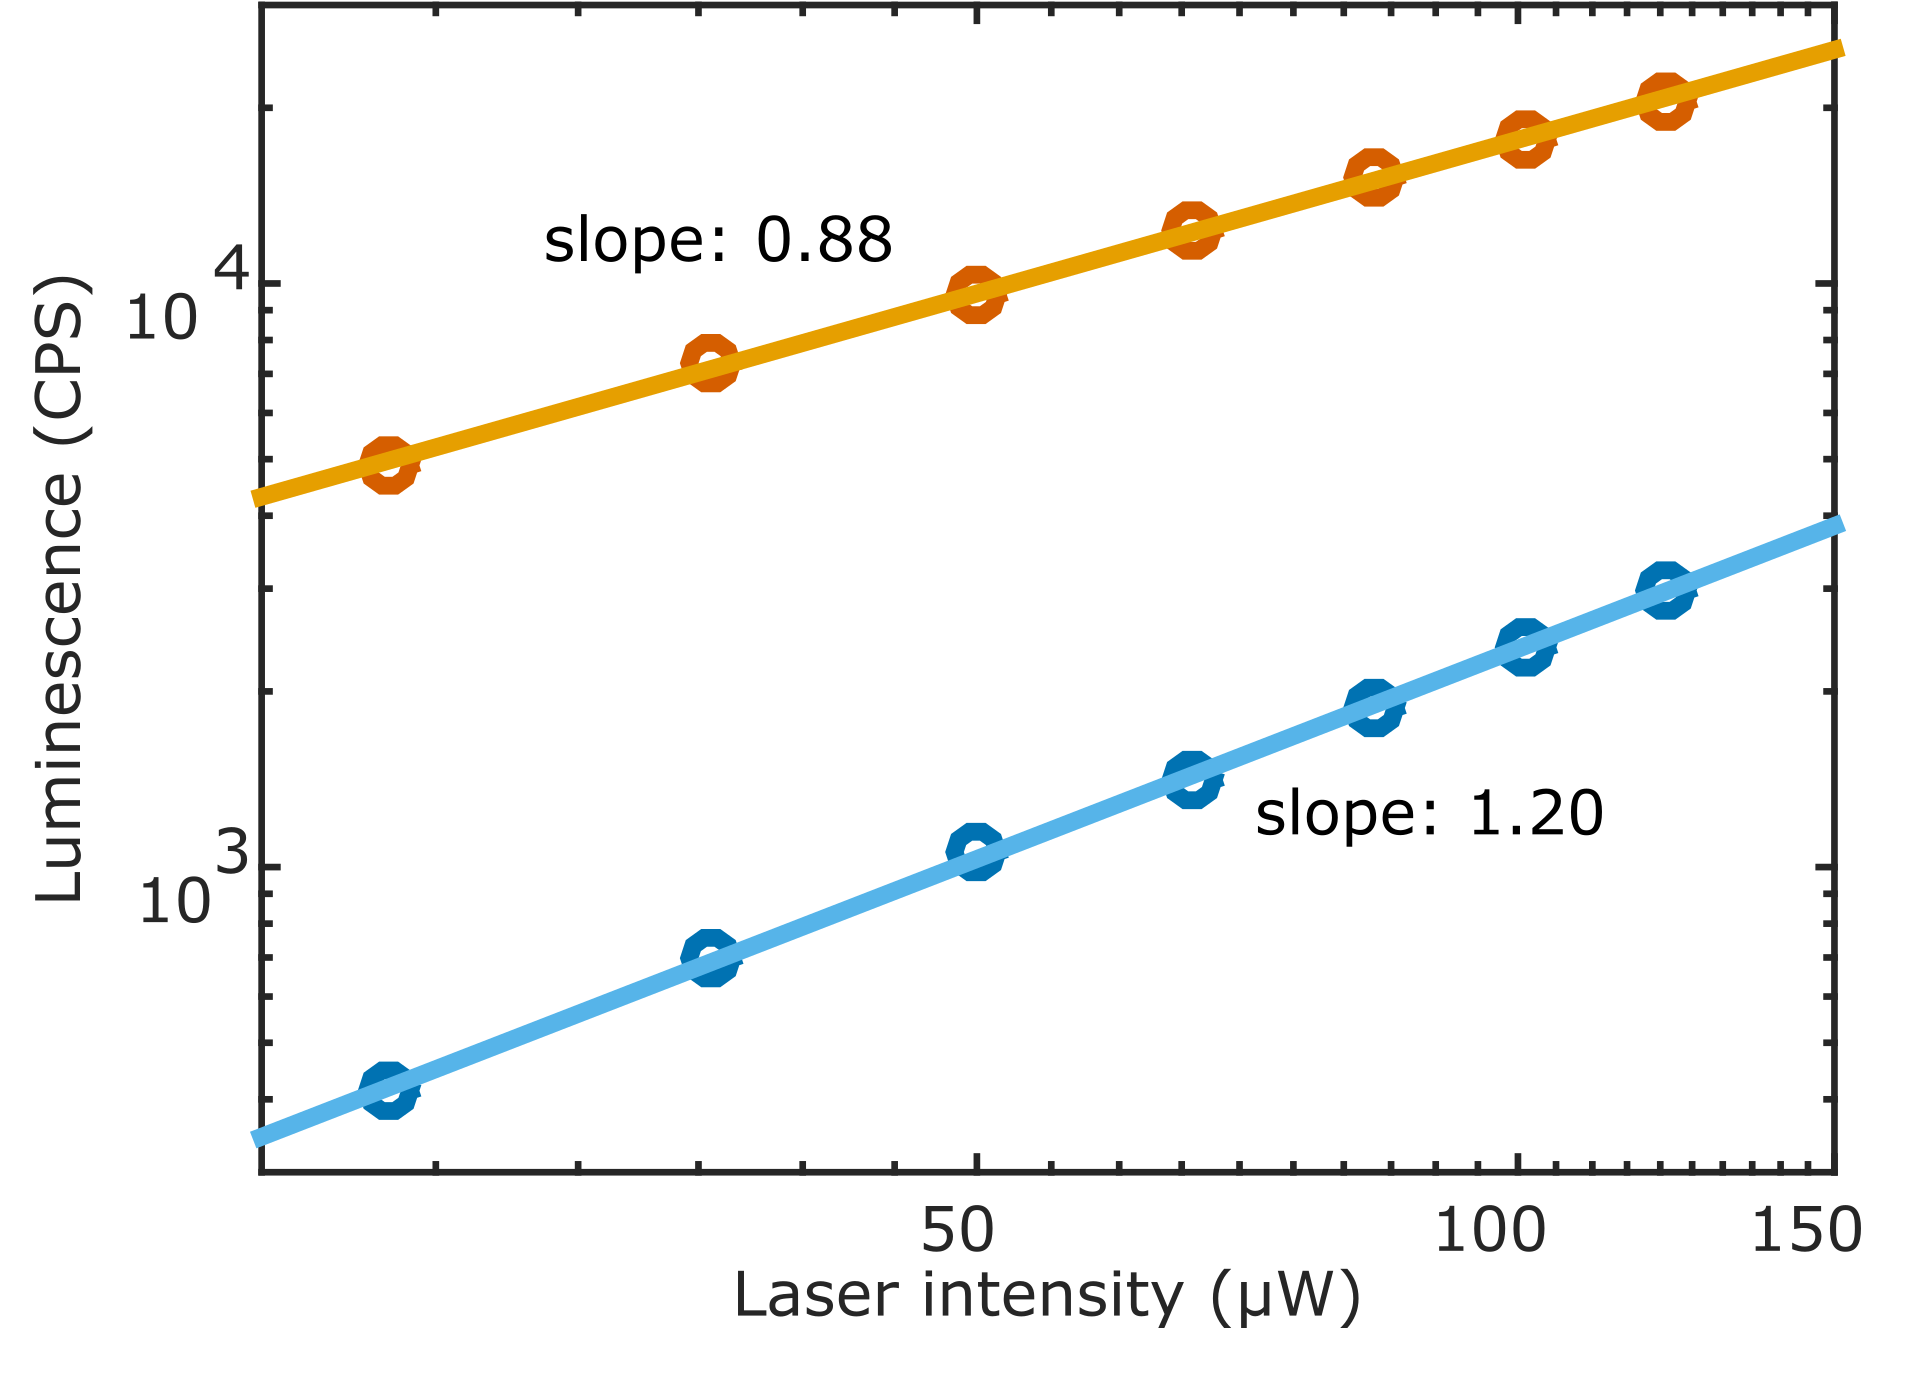
\includegraphics[width=0.45\textwidth]{Figures/Supplementary/01_AS_S_in_Log/01_AS_S_in_Log.png}
\caption{Stokes and anti-Stokes emission as a function of excitation power. The
linear fit in logarithmic scale has a slope of $0.9$ and $1.2$ respectively,
ensuring the 1-photon nature of both kinds of emission.}
	\label{fig:Log_Plot}
\end{figure}

Figure \ref{fig:Log_Plot} shows the intensity of the Stokes (red) and
anti-Stokes (blue) emission for several excitation powers. In both cases the
linear fit in logarithmic scale has a slope close to $1$, being $0.9$ for the
Stokes and $1.2$ for the anti-Stokes, ensuring that both types of emission are
single-photon processes. The behavior is independent of the plasmon resonance
position. It is important to note that the excitation intensity cannot be
increased much beyond what is shown because nanorods would start reshaping into
spheres given enough laser power.

\begin{figure}[htp] \centering
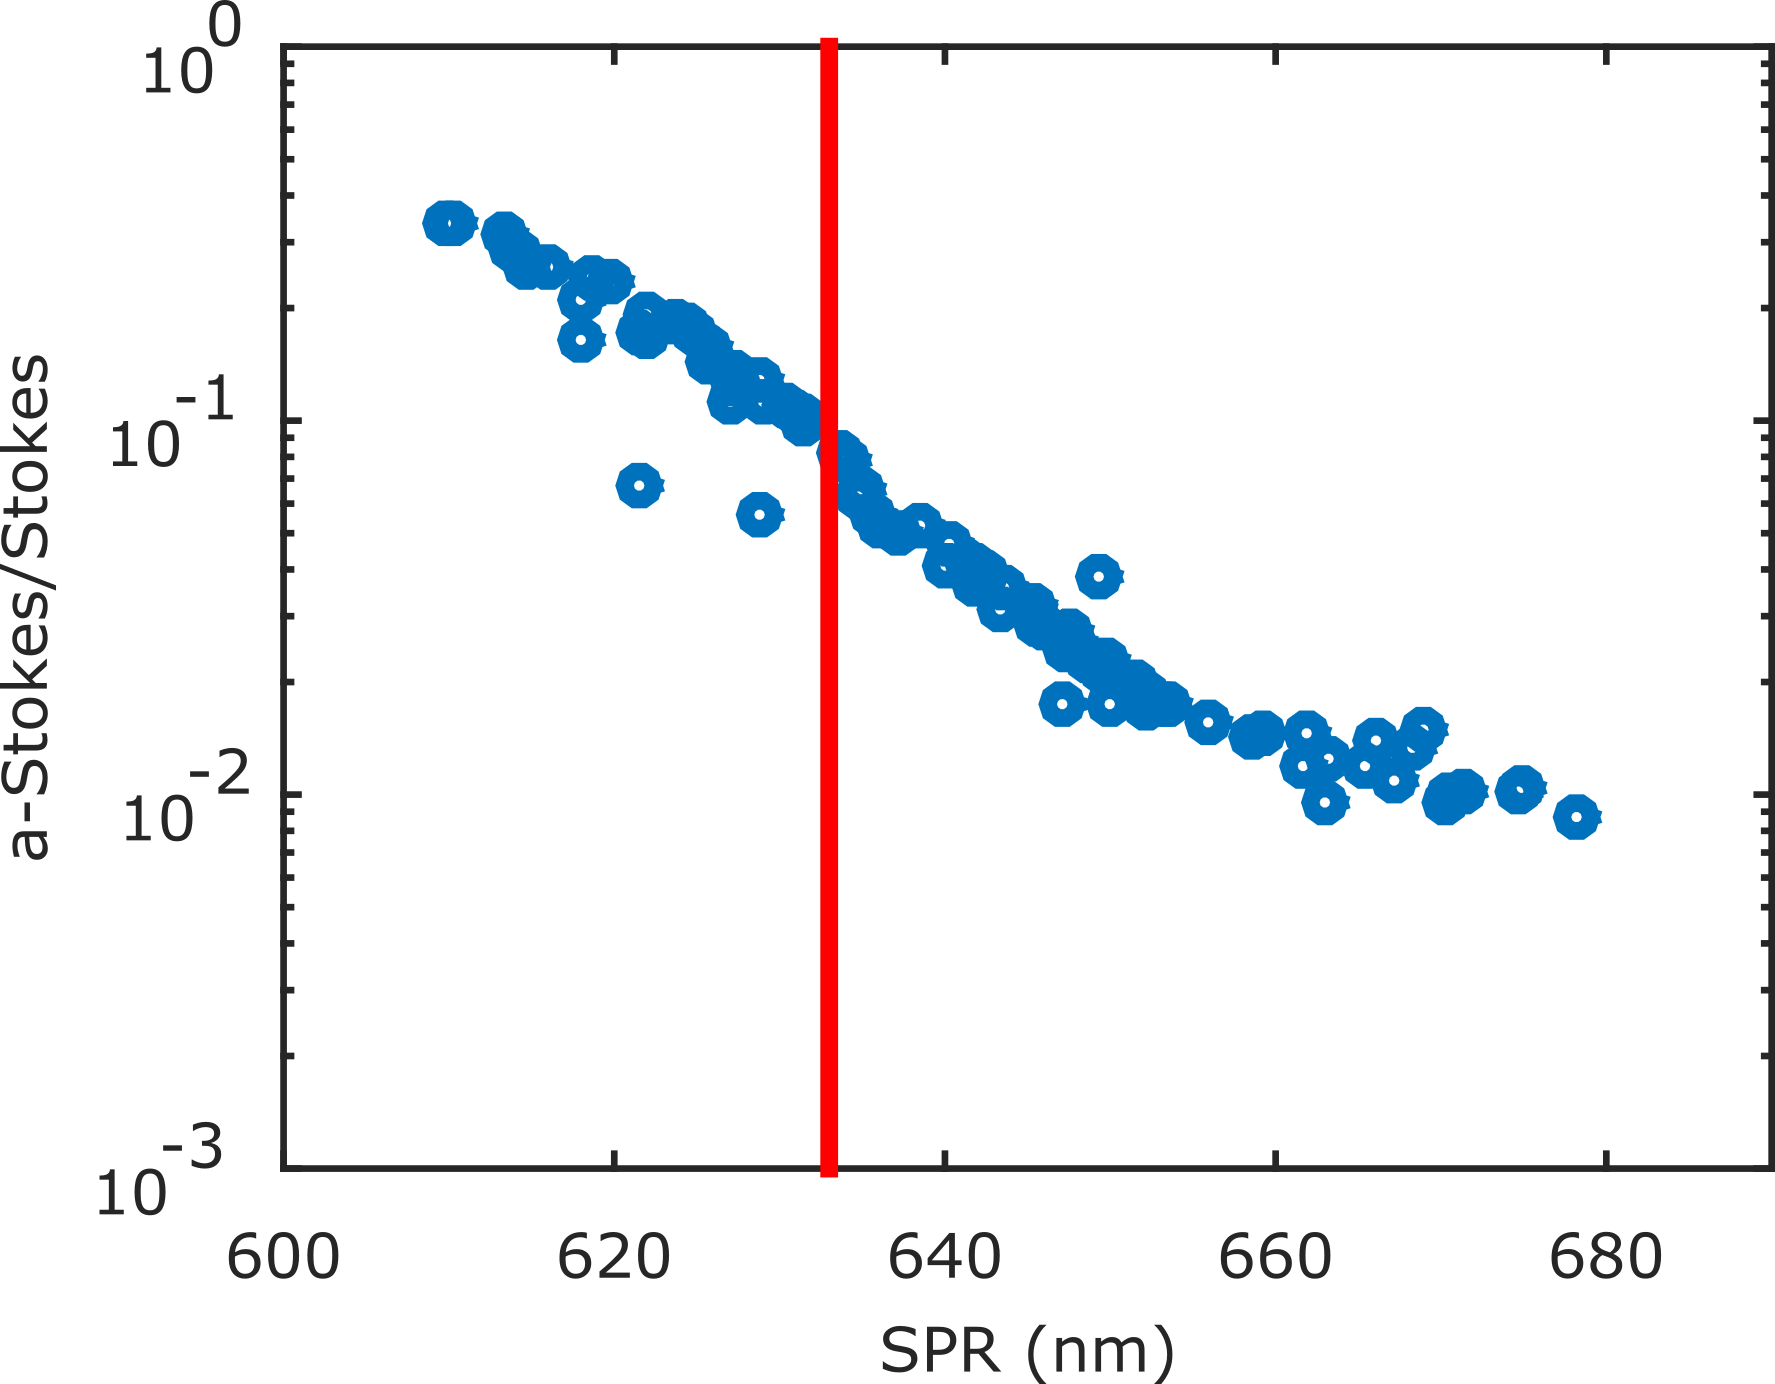
\includegraphics[width=0.45\textwidth]{Figures/Supplementary/02_AS_vs_S_SPR/02_AS_vs_S_SPR.png}
\caption{Ratio of the anti-Stokes to Stokes emission as a function of the
resonance position for 90 different particles under $633\nm$
irradiation at $100\uW$. The red line shows the position of the laser.}
	\label{fig:ASS-ratio}
\end{figure}

Figure \ref{fig:ASS-ratio} shows the ratio of the anti-Stokes emission to the
Stokes emission for $90$ nanorods with different plasmon resonance and under the
same $633\nm$ excitation. The vertical red line depicts the laser wavelength. It
can be seen that the maximum ratio happens when the laser is red-detuned from
the resonance. This is the case where the plasmon is enhancing preferably the
anti-Stokes emission. It has to be kept in mind that off-resonance the cross
section is lower and therefore the excitation is not as efficient. Particles
with a resonance at the laser wavelength in which nor the anti-Stokes nor the
Stokes is preferred, show a ratio close to $10\%$.

\begin{figure}[htp] \centering
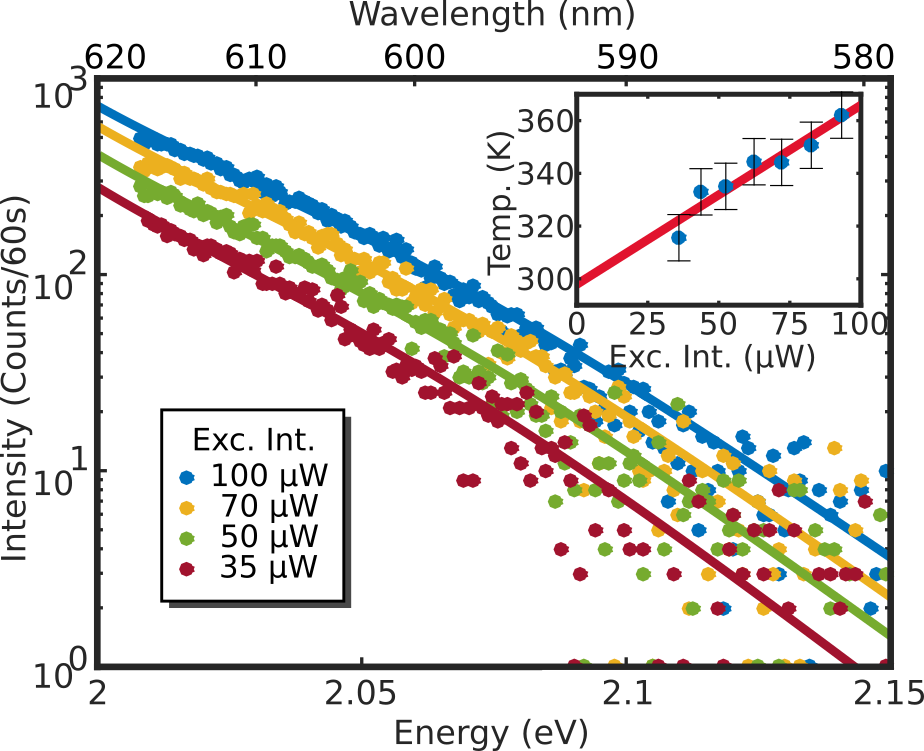
\includegraphics[width=0.45\textwidth]{Figures/03_Fit_Of_AS/03_Log_Fit_AS.png}
\caption{Anti-Stokes emission at different irradiation powers with the
corresponding fitting by equation \ref{eqn:fitting}. There is a good overlap
between data and model. The inset shows the extracted temperature at each
power (blue dots) and a linear extrapolation of the data to $0\uW$ excitation
power. The value obtained for room temperature was $293\K$ while the measured
value was $296\K$. The green stars are the calculated temperatures under the
same excitation conditions. There is a good agreement between experimental and
numerical values.}
	\label{fig:AS_in_Log}
\end{figure}

By fitting the anti-Stokes part of the spectra shown in \ref{fig:spectra_rod}
with the equation \ref{eqn:fitting} it is possible to extract the temperature of
the particle at each excitation power. Figure \ref{fig:AS_in_Log} shows the
result of this procedure. The spectra shown were recorded at $4$ different
excitation intensities; the full lines are the fitting results. There is a good
agreement between the fitting and the experimental values. The inset in the
figure shows the extracted temperatures at different intensities (blue dots).
Firstly is possible to observe that the temperature is proportional to the
excitation intensity and therefore to the absorbed energy, as expected. From
these data is possible to calculate the temperature at $0\uW$ excitation
power, i.e. room temperature, by extrapolating the results of a linear fit. The
obtained value in this case is $293\K$, while room temperature was set to
$296\K$.

To prove that the temperature values obtained with this procedure are
reasonable, we performed finite element analysis using Comsol. The cross section
was obtained from discrete dipole calculations employing the ADDA
package\cite{Yurkin2011}. The values for the dimensions of the particle were
deducted from SEM images, and the length was adjusted to obtain a plasmon
overlapping to the observed one. The inset in Fig. \ref{fig:AS_in_Log} shows the
calculated temperatures under the same excitation conditions as the red stars.
There is a good agreement between both measurements and simulations. Moreover it
can be seen that once calculated the cross section of the particle, the
temperature of a rod or of a sphere with the same volume are the same, therefore
the temperature can be easily determined from the absorbed power using the heat
equation.

As expected from the model, the anti-Stokes emission should depend not only on
the particle intrinsic properties but also on the temperature of the surrounding
medium\cite{Konrad2013}. The samples were mounted in a flowcell that allowed to
change the temperature and to measure it with a Pt100 resitance thermo detector.
It has to be remembered that in this set of experiments we employed a dry
objective, and therefore the excitation powers are larger to compensate for the
lower excitation efficiency. At each temperature several spectra were acquired
at different $633\nm$ excitation powers and also a spectrum of the plasmon
before and after in order to monitor any possible reshaping of the particles
during the experiment.

\begin{figure}[htp] \centering
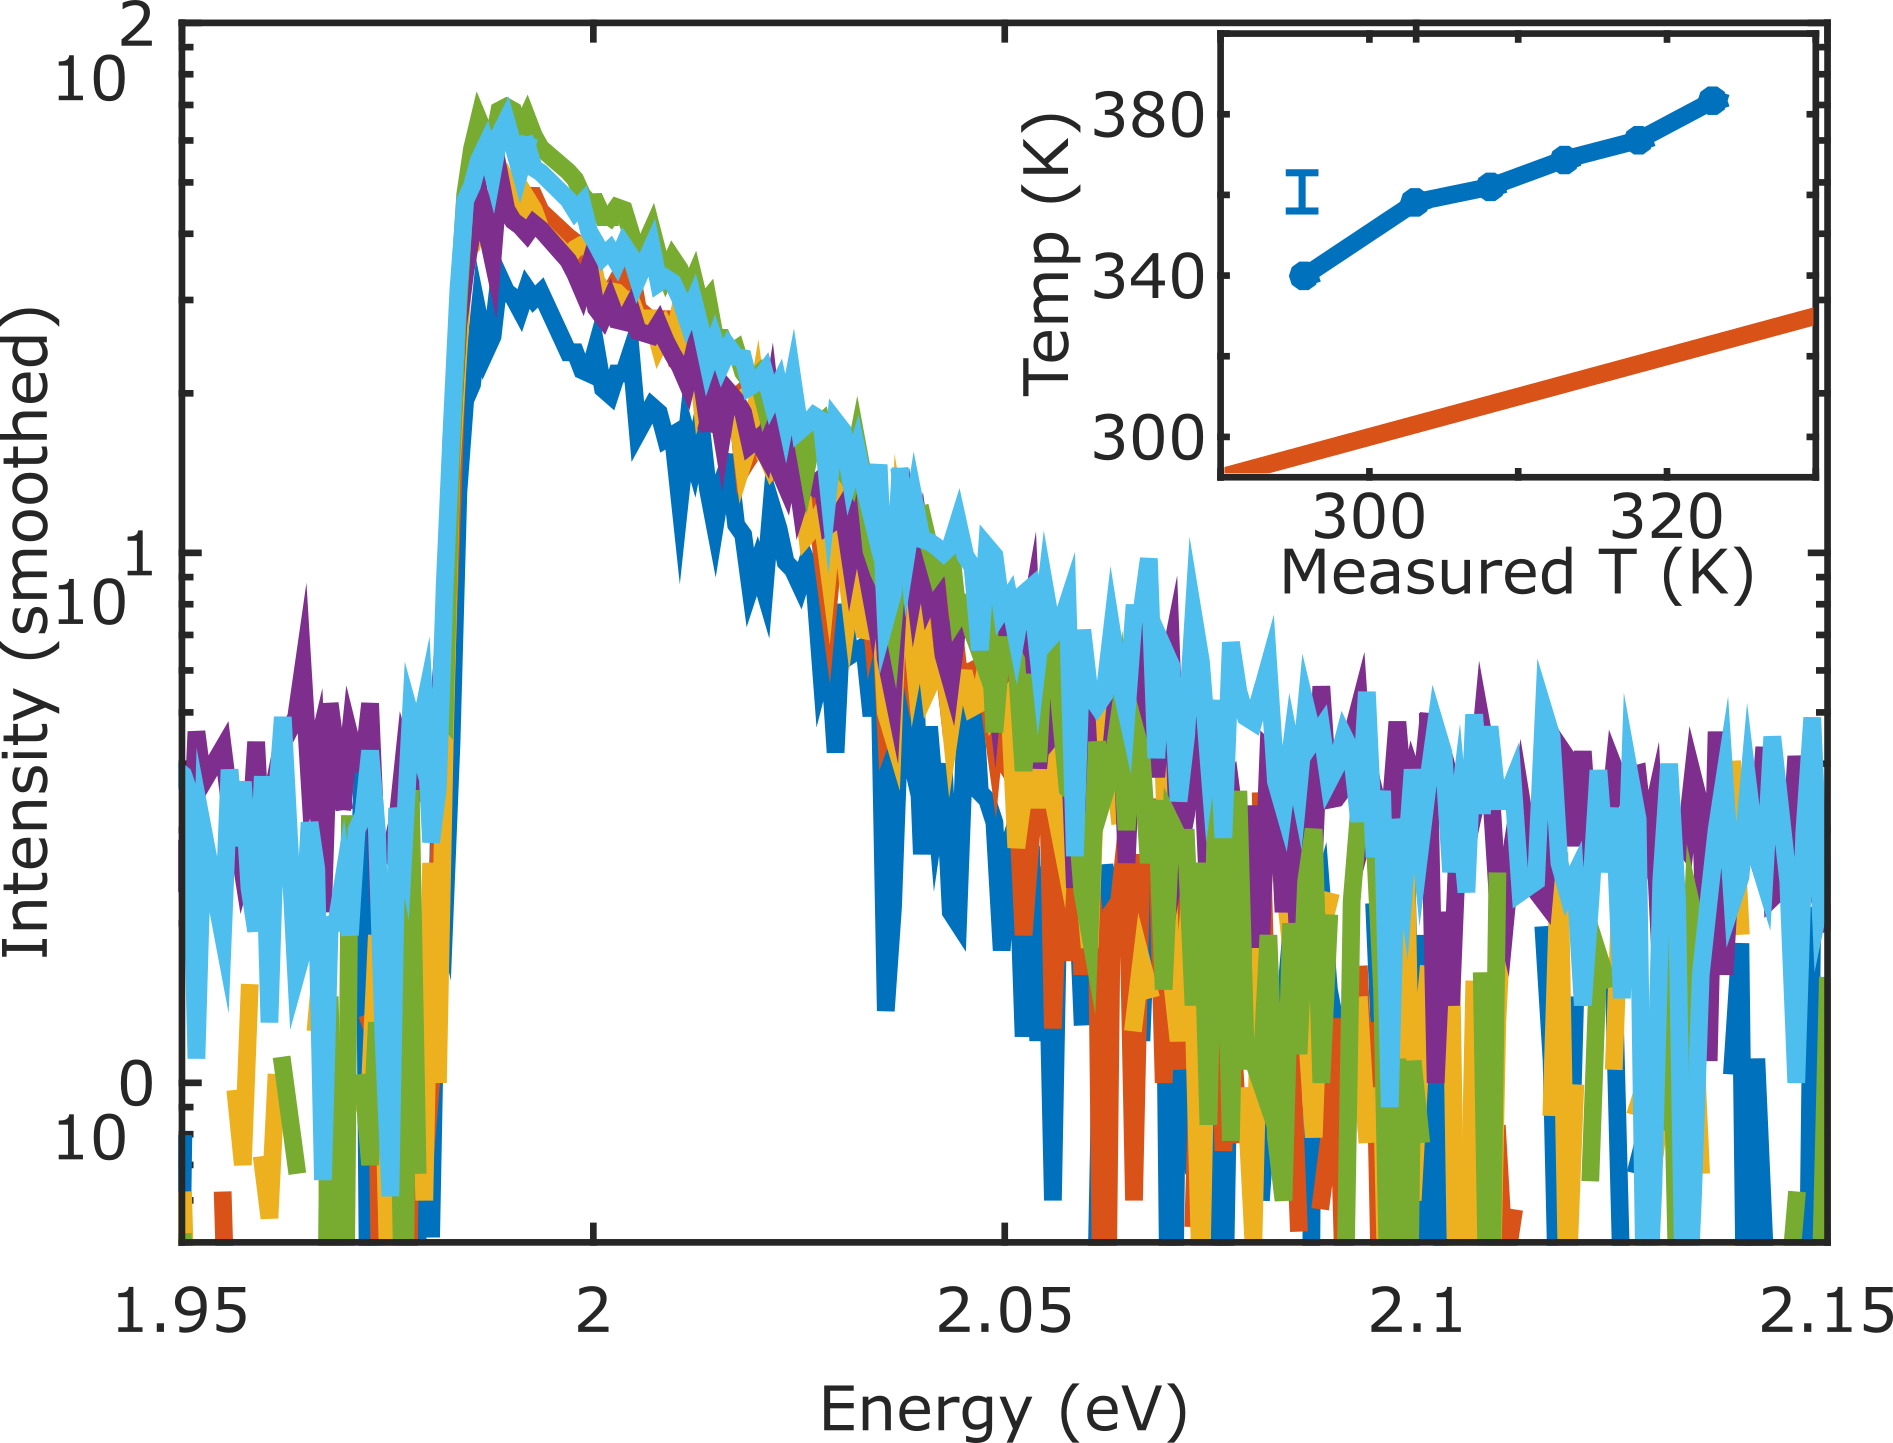
\includegraphics[width=0.45\textwidth]{Figures/04_Extracted_Temp/04_extracted_temp.png}
\caption{Anti-Stokes emission spectra under $633\nm$ laser excitation at
$510\uW$ but at different temperatures. The inset shows the extracted
temperature as the temperature of the medium increases.}
	\label{fig:AS-temps-rods}
\end{figure}

Figure \ref{fig:AS-temps-rods} shows the anti-Stokes emission spectra at
$510\uW$ but at different temperatures. The changes in the slope of the curves
encode the different temperatures. The inset in Fig. \ref{fig:AS-temps-rods}
shows the extracted temperature from the fitting with equation \ref{eqn:fitting}
as a function of the temperature measured by the Pt100 in the vicinity of the
nanorod. The red line is showing the water temperature and acts as a guide to
the eye.

The inset of Figure \ref{fig:AS-temps-rods} clearly shows an increase in the
extracted temperature while increasing the temperature of the surrounding
medium. The range of explored temperatures was from $296\K$, room temperature,
up to $320\K$. This range is enough to observe a change in the anti-Stokes
emission spectrum. At higher temperatures the stability of the setup
plays a crucial role in maintaining the particle in focus during the spectra
acquisition time. Longer exposure times and therefore lower excitation
intensities can be obtained if particles are actively maintained in focus.

Together with the excitation intensity, the plasmon position has a crucial role
in the accuracy of the extracted temperature. The luminescence spectrum acquired
with the $532\nm$ laser shows an asymmetric shape, due to a broadband
contribution from gold added to the plasmonic emission. This makes the initial
fitting needed for the SPR function of equation \ref{eqn:fitting} non univocally
determined. For the particle shown in Fig. \ref{fig:spectra_rod}, changing the
initial wavelength of the fit from $600\nm$ to $640\nm$ yields a significative
difference in the obtained parameters of the lorentzian.

\begin{figure}[htp] \centering
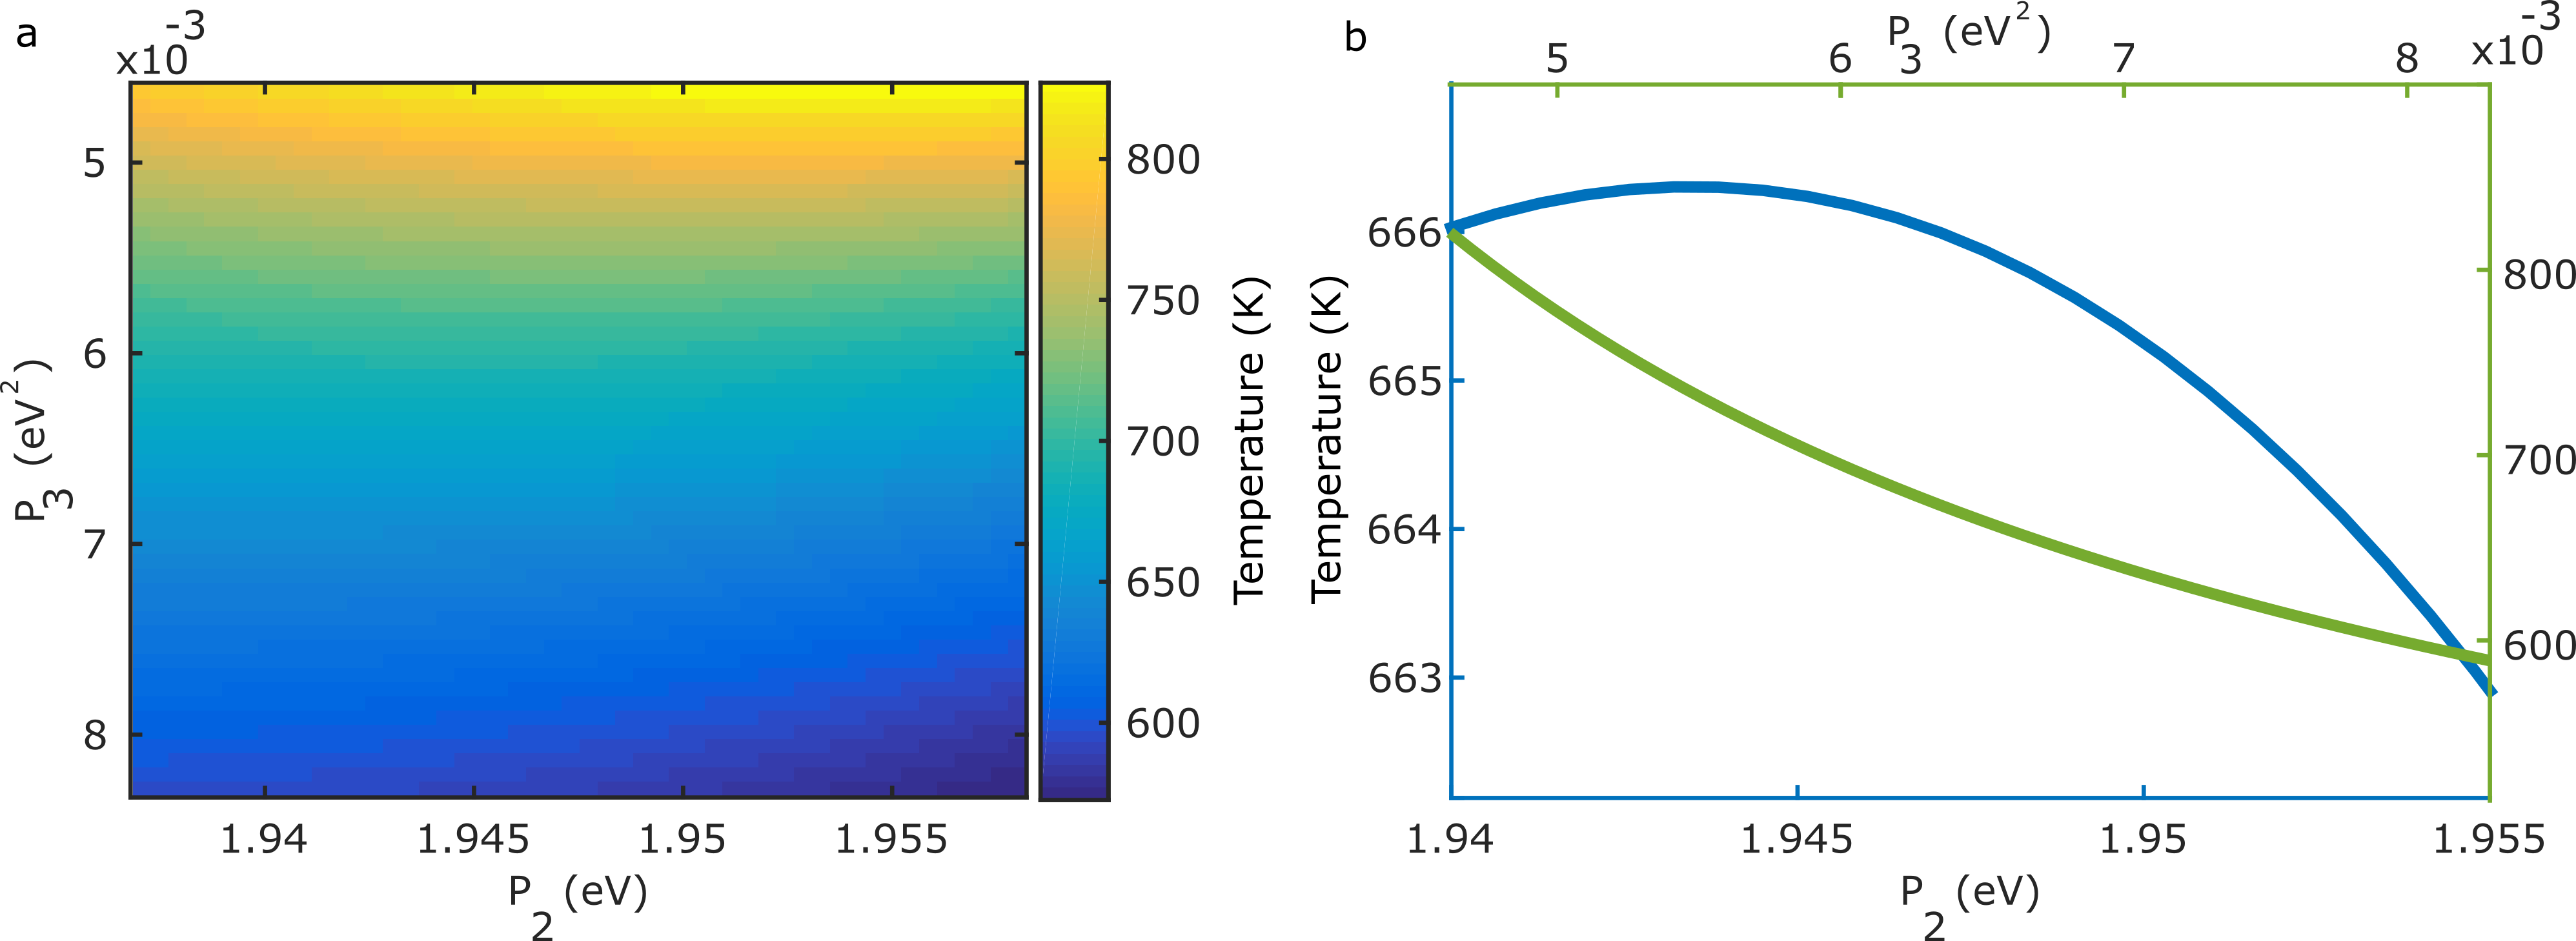
\includegraphics[width=0.90\textwidth]{Figures/05_Estimation_error/05_estimation_error.png}
\caption{Estimation of the error due to different fitting parameters of the
plasmon spectrum. a) 2D grid of the difference in temperature obtained while
varying both $P_2$ and $P_3$ parameters of the fit. b) Temperature dependence
while keeping either $P_2$ or $P_3$ constant.}
	\label{fig:estimation-error}
\end{figure}

Using the following expression for the SPR function in $\eV$, 
\begin{equation*}
\textrm{SPR}(E) = \frac{P_1}{(E-P_2)^2+P_3}
\end{equation*}
The different fitting ranges give values for $P_2$ between $1.940\eV$ and
$1.955eV$, while the values of $P_3$ lie in between $5\cdot10^{-3}\eV^2$ and
$8\cdot10^{-3}\eV^2$. Figure \ref{fig:estimation-error}.a shows the extracted
temperature difference from the anti-Stokes spectra for all the possible
parameter combinations in the range just mentioned. Figure \ref{fig:estimation-error}.b
shows the temperature dependence while keeping either $P_2$ or $P_3$ constant.

In this example it is possible to note that the extracted temperature is highly
dependent on the fitted width of the plasmon spectrum but barely dependent on
the extracted peak position. From the initial spectrum of the particle, it is
possible to note that the wing of the plasmon coincides with the range of
anti-Stokes emission. Therefore minute changes in the initial shape will yield
higher changes in the extracted temperature.

This assertion implies that there should be particles in which the extracted
temperature wouldn't be too sensitive to the initial plasmon fit. To explore
these possibilities, we calculated the anti-Stokes emission of different
particles at $400\K$ by using equation \ref{eqn:fitting} and the results of ADDA
calculations for the SPR function. We then extracted a temperature from these
spectra while varying the lorentzian parameters as was done for the experimental
results. In this way it is possible to study the expected error in temperature
generated by the initial uncertainty in the fitting of the plasmon for different
particles. 

\begin{figure}[htp] \centering
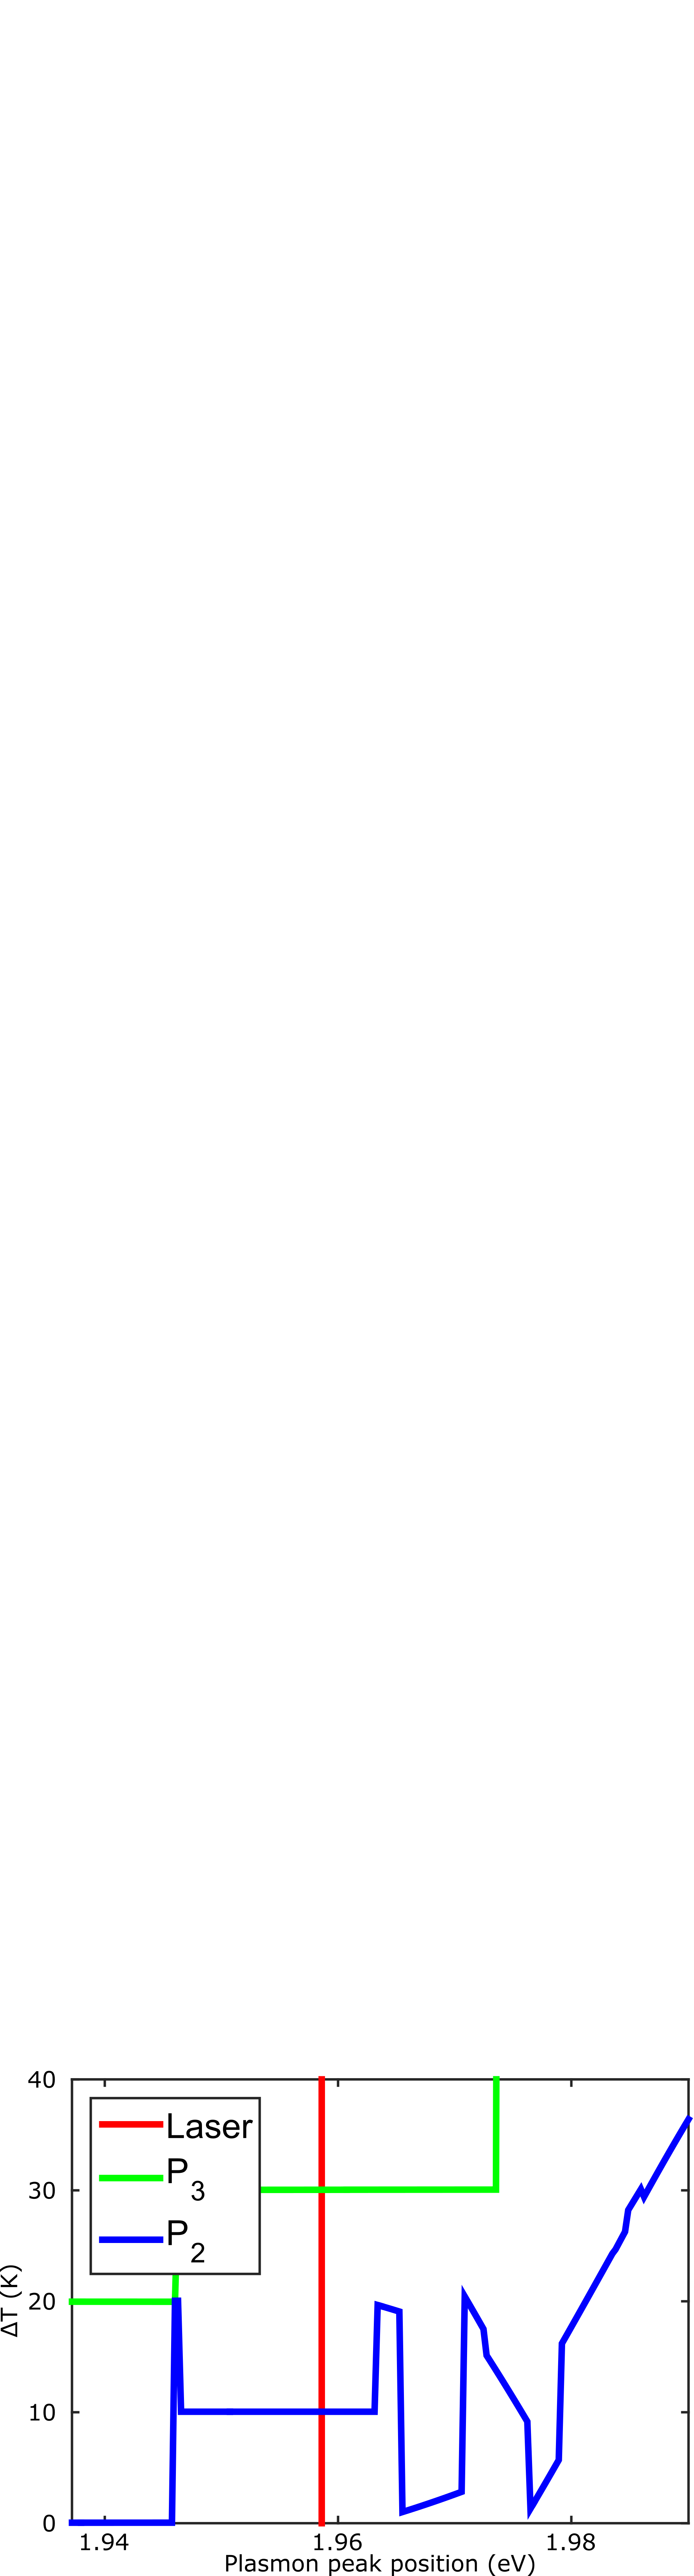
\includegraphics[width=0.45\textwidth]{Figures/06_Calculation_error/06_calculation_error.png}
\caption{Calculated error in the temperature extraction due to the uncertainty
in the plasmon parameters as a function of the resonance position of the
particle. Clearly, when exciting at the blue wing of the plasmon, the effect of
these uncertainties is much lower.}
	\label{fig:calculated-error}
\end{figure}

Figure \ref{fig:calculated-error} shows the uncertainty in the extracted
temperature as a function of the plasmon peak position. The uncertainty is
defined as the difference of the maximum and the minimum extracted temperatures
while varying $P_2$ by $10\%$ and $P_3$ by $30\%$. The vertical red line depicts
the position of the laser. It is remarkable the difference for particles with a
resonance red-shifted from the excitation laser to particles blue-shifted.
Indeed, when the plasmon favors the anti-Stokes emission the correct modelling
of the resonance is crucial for the extraction of temperatures. On the other
hand, when the plasmon is red-shifted from the excitation, the induced error in
the extracted temperature is much lower. The amount of collected light is
another factor to keep into account. When the resonance is red-shifted
from the laser, the anti-Stokes emission is much weaker and therefore
accumulating enough photons in the spectrometers requires longer acquisition
times.

% It was not possible, however, to extrapolate to zero excitation power, since
% only few spectra were clear enough as to proceed with the fitting.

It would be beneficial therefore to have particles that can withstand higher
excitation powers and that have a plasmon resonance well defined. In principle
gold nanospheres fulfill these requirements. They are known to withstand much
higher excitation powers without reshaping nor melting\cite{Hou2015}. Moreover
the plasmon resonance of spheres shifts only slightly with radius, therefore it
is possible to predict it using Mie theory and eliminating the need of a second
laser beam. Sphere samples however always show a shape distribution that cannot
be neglected and that induces a deviation of the observed resonance from the
predicted.

\begin{figure}[htp] \centering
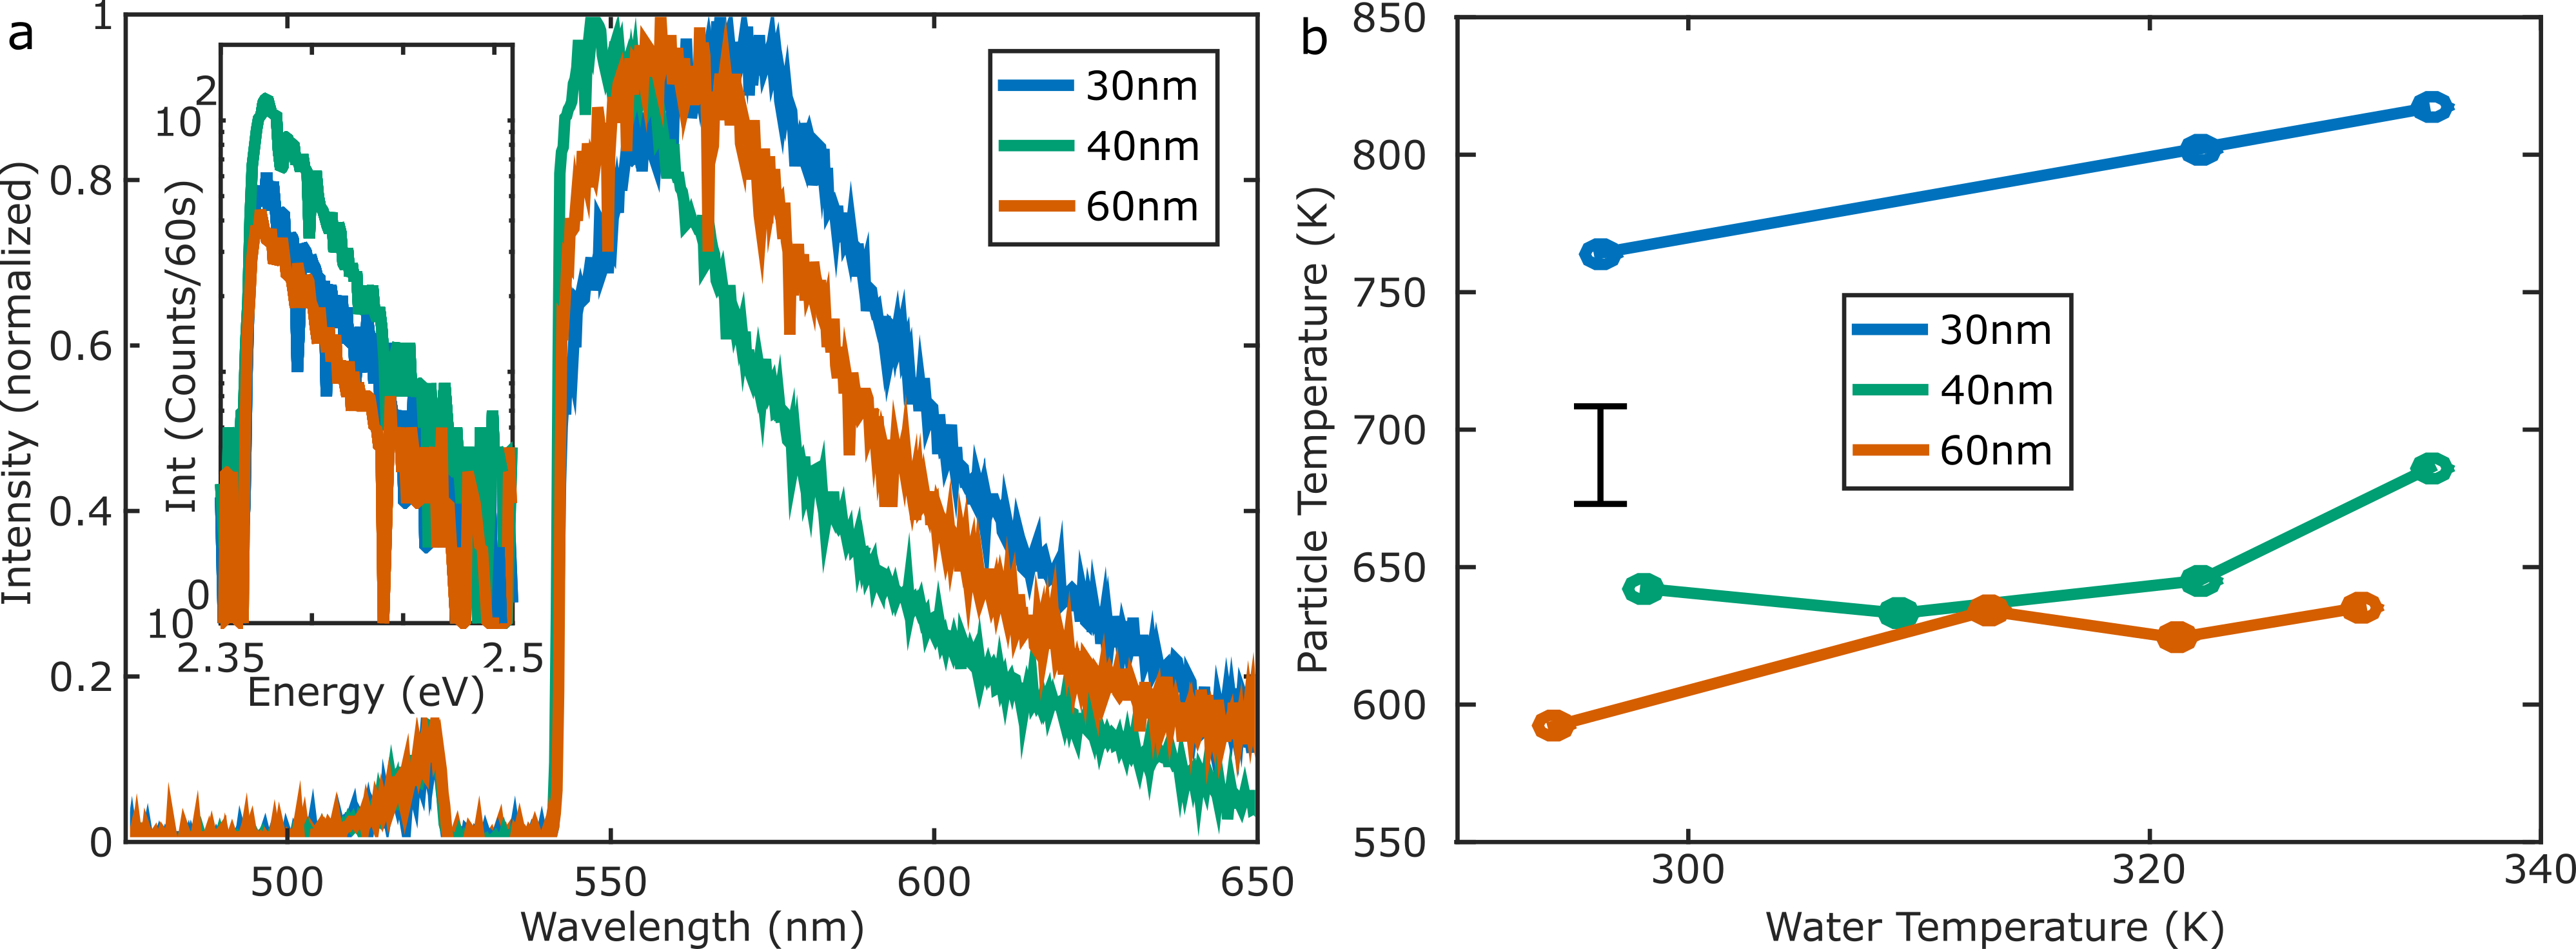
\includegraphics[width=0.90\textwidth]{Figures/07_Spheres/07_spheres.png}
\caption{Spectra and temperature extraction with spheres of
diameter $60\nm$,$40\nm$ and $30\nm$. a) Normalized luminescence spectra of
three particles under $532\nm$ excitation. The inset shows the detail of the
anti-Stokes emission without normalization. The excitation powers for the three
particles were $1.2\mW$, $2.0\mW$ and $3.6\mW$ respectively. b) Extracted
temperature from these particles while increasing the medium temperature.}
	\label{fig:spheres}
\end{figure}

Figure \ref{fig:spheres}.a shows the normalized luminescence spectra of three
nanospheres of diameters $60\nm$, $40\nm$ and $30\nm$ under $532\nm$ excitation.
As for the nanorods, two very distinctive parts of the spectrum are
distinguishable, the Stokes at longer wavelengths and the anti-Stokes at shorter
ones. From Mie theory it would have been expected a blue shift of the resonance
while diminishing the radius of the particles; however the $30\nm$ one seems to
be the more red-shifted. This is most likely due to small anisotropies in the
sample, giving rise to slightly different plasmon resonances. The inset in Fig.
\ref{fig:spheres}.a shows a detail of the anti-Stokes emission for the three
spheres without any further normalization. It has to be pointed out, however,
that the excitation intensity was $1.2\mW$, $2.0\mW$ and $3.6\mW$ to compensate
for the lower cross sections of the smaller particles.

It has to be noted that spheres have not only a smaller cross section than
nanorods of the same volume, but their quantum yield is also one order of
magnitude lower than for rods and it holds true for the anti-Stokes emission.
This can be compensated by increasing the excitation power up to either reaching
a melting temperature of gold or a phase transition of the surrounding liquid
that in turn would induce a shift in the plasmon resonance. This is why the
powers employed with spheres are much higher than the ones employed with rods.

Figure \ref{fig:spheres}.b shows the extracted temperature of the three
particles while increasing the medium temperature. It is possible to see that
the small $30\nm$ diameter sphere is $150\K$ hotter than both the $40\nm$ and
$60\nm$. The three curves show an increasing trend, but in this case the
variation of medium temperature amounts to less than $5\%$ the temperature of
the particles. The extracted temperature is similar to what would be expected
from the heat equation, considering the absorption cross section given by Mie
theory. An analysis on the error similar to the one performed with rods yields a
relative tolerance of about $5\%$ in the extracted temperature, and therefore is
not possible to conclude that the increase in the calculated temperature is in
fact given by the increase in the medium\'s temperature.

\section{Conclusions}
Being able to control and monitor temperature at the nanoscale is of utmost
importance in different fields ranging from photothermal therapy\cite{Huang2006}
to nano fabrication\cite{Fedoruk2013}. In this work we have shown a simple
procedure that allows to measure the temperature of single gold nanorods and
nano spheres while being irradiated under a monochromatic continuous laser. The
level of accuracy on the temperature measurement depends on several factors, but
for nanorods it can be estimated to be better than $2.5\%$ and for nanospheres
around $5\%$.

The model employed for describing the anti-Stokes emission takes into account
the presence of the plasmon, responsible for enhancing the emission as well as
Bose-Einstein statistics to explain the distribution of the exited states of the
particles. It has been shown that the correct characterization of the plasmonic
resonance is fundamental for the proper extraction of temperature, specifically
in the cases where the excitation wavelength is red-detuned from the resonance.

Particles with a resonance to the red of the excitation wavelength would be more
reliable in the temperature extraction procedure, but would also exhibit a lower
emission towards shorter wavelengths. The trade-off between both effects will
determine the specific particles that are better suited for each application.

In this work we have also explored the possibility of employing gold nano
spheres. Since these particles do not reshape under higher excitation powers it
is possible to compensate their lower quantum yield by increasing the
irradiation intensity. Moreover samples with a narrow shape distribution would
be ideal candidates to temperature extraction since their plasmon can be
determined from Mie theory with only one needed parameter, the radius of the
particle.

We have observed the anti-Stokes emission from particles with three different
diameters. The extracted temperature in each case matches with the expected
value from thermal conductivity calculations, but the change when increasing the
surrounding medium temperature falls between the experimental error of the
procedure.

The main advantage of the proposed method is that it doesn't require any
modification or adaptation to existing setups that are capable of recording
emission spectra. Moreover there is no need of calibration, since the only free
parameter of the model is the absolute temperature of the nanoparticle under
study. A $2.5\%$ accuracy in temperature may suffice for several applications.
This value can be improved in different ways: by carefully selecting the
particles that show the most favorable plasmon resonance; by determining the
plasmon resonance through white-light scattering, avoiding the uncertainty in
the parameters; also an ad-hoc calibration of the temperature can be
performed.

\bibliography{anti_stokes}
\end{document}
